\subsection{The ideal-tetrahedron normalization}
\label{sm:local-cells}

We use upper half-space with ideal boundary
$\CC\cup\{\infty\}$. A geodesic plane is vertical over a line or
is a hemisphere orthogonal to the boundary plane. A horizontal
horosphere at $\infty$ has a Euclidean induced metric up to scale.
For positive $a,b,c$ with $a+b+c=1$, the classical volume of
an ideal tetrahedron with dihedral angles $\pi a,\pi b,\pi c$ is
\begin{equation}\label{sm:tetra}
 \begin{split}
 V(a,b,c)&=\Lambda(\pi a)+\Lambda(\pi b)+\Lambda(\pi c)
              =-\pi\{J(a)+J(b)+J(c)\},\\
 \Lambda(t)&=-\int_0^t\log(2\sin u)\,\dd u .
 \end{split}
\end{equation}
We import this normalized local formula, including its continuous
zero value at a flat tetrahedron, from classical hyperbolic
geometry \cite{Milnor}. All cell volumes below are ordinary sums
of positive tetrahedron volumes.

\subsection{The leaf pyramid}
For $0<a<1/2$, put $E=e^{2\pi\ii a}$. The convex hull of
\begin{equation}\label{sm:leaf}
 O=\infty,\qquad (C_0,C_1,C_2,C_3)=(1,E,-1,-E)
\end{equation}
is an ideal quadrangular pyramid. Its four finite vertices form
a rectangle. Its side planes are vertical over the four rectangle
edges; its base plane is the unit hemisphere. These five
supporting planes enclose exactly the convex hull. Adjacent
vertical planes meet at right angles, so every apex edge has
angle $\pi/2$.

Call base edges $01,23$ free and $12,30$ cap edges. Intersecting
a vertical chord plane with the unit hemisphere gives interior
angle equal to half the angle subtended by that chord at the
circle center. Thus free edges have angle $\pi a$, and cap
edges have angle $\pi(1/2-a)$.
Color $(O,C_1,C_2)$ and $(O,C_3,C_0)$ shaded and the other two
side triangles white. The shaded faces will retain the two
sides of the original half crossing disk. The ordered
quadrilateral base is a gluing face in the cut construction.

The diagonal $C_0C_2$ divides the pyramid into two positive
tetrahedra with angle triple $(a,1/2-a,1/2)$. By
\eqref{sm:tetra},
\[
 \Vol(\text{leaf})=2V(a,1/2-a,1/2)=\pi g(a).
\]
The last equality follows either by differentiating the two
expressions and evaluating at $a=0$, or from
$J(2a)=2J(a)-2J(1/2-a)$.

\begin{figure}[ht]
\centering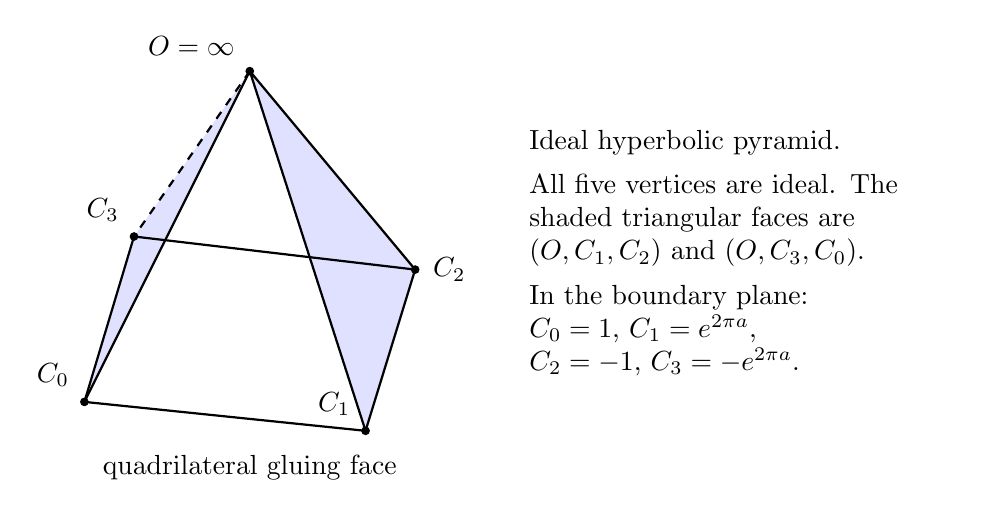
\begin{tikzpicture}[scale=1.05]
\coordinate (c0) at (-2,-1);\coordinate(c1) at (1.4,-1.35);\coordinate(c2) at (2,.6);\coordinate(c3) at (-1.4,1);\coordinate(o) at (0,3);
\fill[blue!12] (o)--(c1)--(c2)--cycle;\fill[blue!12] (o)--(c3)--(c0)--cycle;
\draw[thick] (c0)--(c1)--(c2)--(c3)--cycle;
\draw[thick] (o)--(c0) (o)--(c1) (o)--(c2);\draw[thick,dashed] (o)--(c3);
\foreach \p/\l in {c0/C_0,c1/C_1,c3/C_3,o/O=\infty}{\fill (\p) circle(1.5pt);\node[above left=2pt] at (\p) {$\l$};}
\fill (c2) circle(1.5pt);\node[right=3pt] at (c2) {$C_2$};
\node at (0,-1.8) {quadrilateral gluing face};
\node[align=left,text width=5.5cm] at (6,.8) {Ideal hyperbolic pyramid.\\[4pt]All five vertices are ideal. The shaded triangular faces are $(O,C_1,C_2)$ and $(O,C_3,C_0)$.\\[4pt]In the boundary plane:\\ $C_0=1$, $C_1=e^{2\pi\ii a}$,\\ $C_2=-1$, $C_3=-e^{2\pi\ii a}$.};
\end{tikzpicture}

\caption{The ideal hyperbolic leaf pyramid. The two shaded
triangles record the sides of a half crossing disk. The ordered
quadrilateral is a gluing face of the cut cells; it is not
identified with the physical four-punctured boundary of a
tangle box.}\label{sm:leaf-figure}
\end{figure}

\subsection{The multiplication prism}
Given a strict product, put
$p=z-x$, $q=z-y$, $r=x+y-z$, $w=1-x-y$.
All four numbers are positive, and $p+q+2r+w=1$.
Choose four points on the unit circle:
\begin{equation}\label{sm:prism-vertices}
 v_0=1,\qquad v_1=e^{2\pi\ii p},\qquad
 v_2=e^{2\pi\ii(p+r)},\qquad
 v_3=e^{2\pi\ii(p+r+q)}.
\end{equation}
Their successive half-arcs are $p,r,q,r+w$.
The extended chords $v_0v_1$ and $v_3v_2$ meet at a point $P$.
The triangle $(P,v_1,v_2)$ has angles $\pi w,\pi y,\pi x$
at those respective vertices. The sine rule, with chord lengths
$2\sin\pi p$, $2\sin\pi q$, $2\sin\pi r$, gives
\begin{equation}\label{sm:prism-P}
 \begin{split}
 P&=v_1+
 \frac{\sin\pi x\sin\pi r}{\sin\pi w\sin\pi p}(v_1-v_0)\\
  &=v_2+
 \frac{\sin\pi y\sin\pi r}{\sin\pi w\sin\pi q}(v_2-v_3).
 \end{split}
\end{equation}
Both coefficients are positive. Thus the orders on the two
lines are $v_0,v_1,P$ and $v_3,v_2,P$.

Attach the tetrahedron $(\infty,P,v_1,v_2)$ to the pyramid
$(\infty,v_0,v_1,v_2,v_3)$ across $(\infty,v_1,v_2)$.
Their interiors lie on opposite sides of that vertical plane.
The faces over $v_0v_1$ and $v_1P$ are coplanar, as are those
over $v_3v_2$ and $v_2P$. Merging them leaves three quadrilateral
faces and two triangular faces:
\[
 \begin{gathered}
 F_x=(\infty,v_0,v_1,P),\qquad
 F_y=(\infty,v_3,v_2,P),\qquad F_z=(v_0,v_1,v_2,v_3),\\
 (P,v_1,v_2),\qquad(\infty,v_0,v_3).
 \end{gathered}
\]
The last two faces are white.

There are five supporting planes: the vertical planes over
$v_0v_1$, $v_2v_3$, $v_3v_0$, and the hemispheres over the
circles $(v_0,v_1,v_2,v_3)$ and $(P,v_1,v_2)$.
The power of $P$ with respect to the unit circle is positive,
because $P$ is beyond $v_1$ on the chord $v_0v_1$.
Likewise the powers of $v_0,v_3$ with respect to the circle
$(P,v_1,v_2)$ are positive: along its two secants the points
have orders $v_0,v_1,P$ and $v_3,v_2,P$.
Consequently both attached pieces are in the same inward
half-space of each of these five planes. Their union is the
convex ideal triangular prism bounded by those faces.
This proves support and nonintersection throughout the strict
domain, rather than for one drawn example.

\begin{figure}[ht]
\centering\begin{tikzpicture}[scale=2.1, every node/.style={font=\small}]
\coordinate(v0) at (1,0);
\coordinate(v1) at ({cos(43.2)},{sin(43.2)});
\coordinate(v2) at ({cos(79.2)},{sin(79.2)});
\coordinate(v3) at ({cos(140.4)},{sin(140.4)});
\coordinate(P) at (0.57935,1.06242);
% Exact intersection of the two extended chords is used below.
\path[name path=first] (v0)--($(v0)!3!(v1)$);
\path[name path=second] (v3)--($(v3)!3!(v2)$);
\path[name intersections={of=first and second,by=P}];
\draw[gray] (0,0) circle(1);
\fill[blue!10] (P)--(v1)--(v2)--cycle;
\draw[thick] (v0)--(P)--(v3)--cycle;
\draw[thick] (v0)--(v1)--(v2)--(v3);
\draw[dashed] (v1)--(v3);
\foreach \p/\lab/\pos in {v0/v_0/right,v1/v_1/right,v2/v_2/left,v3/v_3/left,P/P/above}
 {\fill (\p) circle(.7pt);\node[\pos=2pt] at(\p){$\lab$};}
\node at (0,-1.3) {$p=.12,\quad r=.10,\quad q=.17,\quad w=.51$};
\node[align=left,text width=5.2cm] at (2.6,.3) {Boundary-plane construction.\\[3pt]$P=(v_0v_1)\cap(v_2v_3)$ lies outside the unit circle.\\[3pt]The sixth ideal vertex is $\infty$. The three quadrilateral gluing faces have ordered vertices $(\infty,v_0,v_1,P)$, $(\infty,v_3,v_2,P)$ and $(v_0,v_1,v_2,v_3)$.};
\end{tikzpicture}

\caption{Boundary-plane support data for the multiplication
prism; its sixth ideal vertex is $\infty$. The point $P$ is
the intersection of the extended chords, with the two orders
proved in \eqref{sm:prism-P}. The circle through $P,v_1,v_2$
and the unit circle support the two bounded faces.}
\label{sm:prism-figure}
\end{figure}

The original lower and upper attachments and the output order are
\begin{equation}\label{sm:stack-map}
 F:C\mapsto(v_0,v_1,P,\infty),\quad
 G:C\mapsto(\infty,P,v_2,v_3),\quad
 C^o=(v_0,v_1,v_2,v_3).
\end{equation}
Reading angles between the supporting planes gives
\begin{equation}\label{sm:prism-angles}
\begin{array}{c|ccccc}
\text{edge}&Pv_1,\infty v_0&Pv_2,\infty v_3&
v_1v_2,v_0v_3&P\infty&v_0v_1,\ v_2v_3\\\hline
\text{angle}/\pi&x&y&1-z&w&p,\ q
\end{array}.
\end{equation}
For a circle and a chord plane, the dihedral angle is the
opposite inscribed angle. Applied to $(P,v_1,v_2)$ this gives
$x,y$ at $Pv_1,Pv_2$; the angle between the two vertical chord
planes is $\pi w$. At the unit-circle base the half-arcs give
$p,q$. The remaining angles follow at the ideal vertices:
their Euclidean links are triangles, so the interior dihedral
angles sum to $\pi$. For example $x+y+w=1$ at $P$, and
$x+p+(1-z)=1$ at $v_1$. This verifies every row of the table.

Divide the original quadrangular pyramid across $v_0v_2$.
Its tetrahedron triples are $(p,r,1-p-r)$ and
$(p+r,q,r+w)$. In their volumes the terms at $p+r$ and
$1-p-r$ cancel. The attached tetrahedron has triple $(y,x,w)$.
Thus the sum is also
\begin{equation}\label{sm:prism-volume}
 \begin{split}
 \Vol(\text{prism})
 &=V(y,x,w)+V(p,q,2r+w)+V(p+q,r,r+w)\\
 &=\pi m(x,y,z).
 \end{split}
\end{equation}
To check the first rewriting, the two extra terms
$\Lambda(\pi(p+q))$ and $\Lambda(\pi(2r+w))$ cancel because
their arguments sum to $\pi$. For the second equality use
$x=q+r$, $y=p+r$, $z=p+q+r$, $r+w=1-z$ and
$w=1-x-y$ in \eqref{sm:tetra}. All triples used here are
positive and sum to one.

\subsection{Matching the whole ordered face}
For a cyclically ordered ideal quadruple define
\begin{equation}\label{sm:kappa}
 \kap(a,b,c,d)=\frac{(a-b)(c-d)}{(a-d)(b-c)}>0
\end{equation}
with the usual limits at infinity. Sending three vertices
to $(\infty,0,1)$ shows that this positive number determines
the entire ordered ideal quadrilateral, including its shear.
A one-step cyclic shift and a reversal fixing the first
vertex invert $\kap$; full reversal preserves it.

Formula \eqref{sm:prism-P} immediately gives the first two
ratios below as directed ratios on the chord lines; the
third follows from the four unit-circle chord lengths:
\begin{align}
 \kap(F_x)&=\frac{\sin\pi x\sin\pi r}
                    {\sin\pi w\sin\pi p}=e^{-m_x},&
 \kap(F_y)&=\frac{\sin\pi y\sin\pi r}
                    {\sin\pi w\sin\pi q}=e^{-m_y},\label{sm:input-kappa}\\
 \kap(F_z)&=\frac{\sin\pi p\sin\pi q}
                    {\sin\pi z\sin\pi r}=e^{-m_z}.&&\label{sm:output-kappa}
\end{align}
The derivative equalities follow by differentiating the seven
$J$ terms in \eqref{sm:m}; for example
$m_x=\log(\sin\pi w\sin\pi p/(\sin\pi x\sin\pi r))$.
The leaf ratio is $\tan^2(\pi a)=e^{-g'(a)}$.

The lower tuple in \eqref{sm:stack-map} is a cyclic shift of
$F_x$ and the upper is a reversal fixing the first vertex of
$F_y$, so both invert the input ratios. The stationary equations
$f_F'(x)+m_x=0$ and $f_G'(y)+m_y=0$ therefore match all four
ordered vertices of each attachment. The output derivative is
$m_z$, which proves $\kap=e^{-f_E'}$ inductively.
A physical turn cyclically relabels the quadruple and replaces
$b$ by $1-b$, again inverting the ratio.
Finally $C_j^F\mapsto C_{3-j}^G$ is full reversal.
The closing equation $f_F'(b)=f_G'(1-b)$ therefore matches the
whole closing face. None of these steps replaces a complex
shape by its absolute value.
